\documentclass{standalone}
\usepackage{tikz,pgfplots,calc,tkz-euclide}
\usetikzlibrary{positioning,calc}
\usetikzlibrary{arrows}
\usepackage{tkz-euclide}
\usetkzobj{all}


\begin{document}
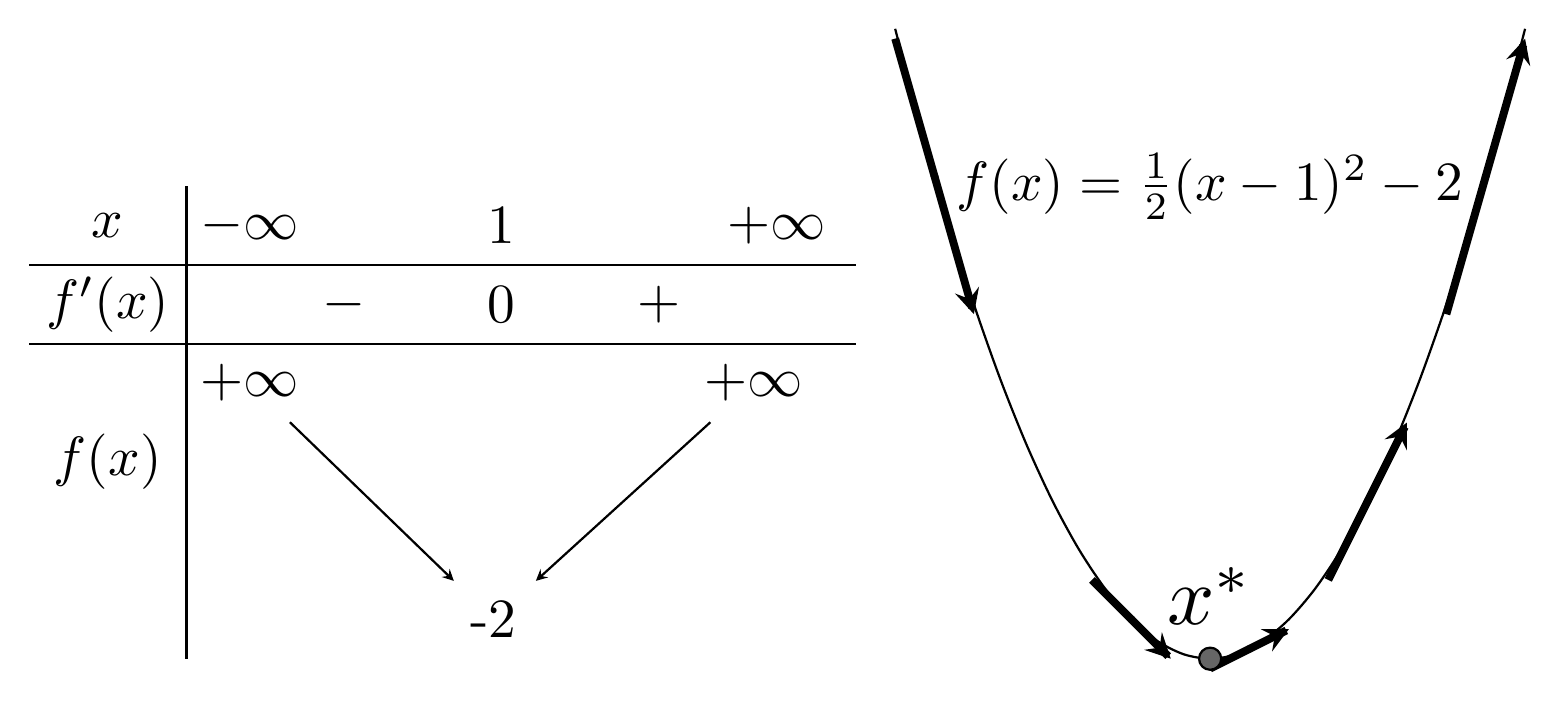
\begin{tikzpicture}[>=stealth, thick]
    \draw (0, 0)  --  ++ (10.5, 0);
    \draw (0, -1)  --  ++ (10.5, 0);
    \draw (2, 1)  --  ++(0, -6);

    \node [scale = 2] at (1, 0.5) {$x$};
    \node [scale = 2] at (1, -0.5) {$f'(x)$};
    \node [scale = 2] at (1, -2.5) {$f(x)$};
    
    \node [scale = 2] at (2.8, .5) {$-\infty$};
    \node [scale = 2] at (6, .5) {$1$};
    \node [scale = 2] at (9.5, .5) {$+\infty$};

    \node [scale = 2] at (6, -.5) {$0$};
    \node [scale = 2] at (4, -.5) {$-$};
    \node [scale = 2] at (8, -.5) {$+$};

    \node (n1) [scale = 2] at (2.8, -1.5) {$+\infty$};
    \node (n3) [scale = 2] at (9.2, -1.5) {$+\infty$};
    \node (n2) [scale = 2] at (5.9, -4.5) {-2};

    \draw [->] (n1)  --  (n2);
    \draw [->] (n3)  --  (n2);


    % graph
    \begin{scope}[xshift = 14cm, yshift = -3cm, scale = 1]
        \draw[domain=-3:5,smooth,variable=\x,black] plot ({\x},{.5*(\x-1)^2-2});      
        \node [scale = 2] at (1, 4) {$f(x) = \frac{1}{2}(x-1)^2 - 2$};
        \foreach \xx in {-0, -2.5, 1.5, 3, 4.5}{
            \draw [fill = black] (\xx, {.5*(\xx - 1)^2 - 2}) circle (1pt);
            \draw[->, black, line width = 1mm, domain=(\xx-.5):(\xx+.5),smooth,variable=\x] plot ({\x},{(\xx - 1)*(\x - \xx) + .5*(\xx - 1)^2 - 2});      
        }
        \draw [fill = gray!80!black, draw = black] (1, -2) circle (4pt);
        \node [scale = 3] at (1, -1.2) {$x^*$};
    \end{scope}

    % \draw[domain=-3:-2] plot (\x,{(\x-1)*(\x-1)-2}) {[turn] (-3,) coordinate(t1) (-1,0) coordinate(t2)};
    % \draw[domain=-2:2] plot (\x,{(\x-1)*(\x-1)-2});
    % \draw[red] (t1) -- (t2);


\end{tikzpicture}
\end{document}